%==============================================================================
%  Amazon Urun Yorumlarinda Uc Sinifli Duygu Analizi - IEEE Konferans Raporu
%  Derleme: Overleaf > Compiler: pdfLaTeX. Gorseller "img/" klasorunde olmali.
%==============================================================================
\documentclass[conference]{IEEEtran}
\IEEEoverridecommandlockouts

\usepackage[T1]{fontenc}
\usepackage[utf8]{inputenc}
\usepackage[turkish]{babel}
\usepackage{graphicx}
\usepackage{float}      % [htbp] -> figür/tabloyu tam metindeki yerine sabitler
% GÜVENLİK AĞI: her görsel otomatik olarak sütun genişliği x sayfa yüksekliğinin
% %42'si kutusuna sığar; figür kodunda boyut yazılmasa bile asla taşmaz.
\setkeys{Gin}{width=\linewidth,height=0.42\textheight,keepaspectratio}
% Görsellerin metin akışına daha iyi oturması ve aradaki beyaz boşlukların
% azaltılması için float yerleşim parametreleri gevşetildi.
\renewcommand{\topfraction}{0.92}
\renewcommand{\bottomfraction}{0.9}
\renewcommand{\textfraction}{0.06}
\renewcommand{\floatpagefraction}{0.75}
\setcounter{topnumber}{3}
\setcounter{bottomnumber}{2}
\setcounter{totalnumber}{5}
\usepackage{booktabs}
\usepackage{array}
\usepackage{amsmath}
\usepackage{amssymb}
\usepackage{textcomp}
\usepackage{xcolor}
\usepackage{url}
\usepackage{hyperref}
\hypersetup{colorlinks=true,linkcolor=black,citecolor=black,urlcolor=blue}

\graphicspath{{img/}{./}}

% IEEEtran anahtar kelime etiketini Türkçeleştir ("Index Terms" -> "Anahtar Kelimeler")
\renewcommand{\IEEEkeywordsname}{Anahtar Kelimeler}

% Yesil delta degeri
\newcommand{\dpos}[1]{\textcolor[rgb]{0.10,0.49,0.13}{\textbf{#1}}}
% Gorsellerin kapladigi alani sinirli tutmak icin standart genislikler
\newcommand{\figS}{0.62\columnwidth}   % kucuk
\newcommand{\figM}{0.82\columnwidth}   % orta
\newcommand{\figL}{0.95\columnwidth}   % genis (tek sutun)

\begin{document}

\title{Amazon Ürün Yorumlarında Üç Sınıflı Duygu Analizi: Klasik, Derin ve Transformer Tabanlı Modellerin Karşılaştırmalı Değerlendirmesi}

\author{\IEEEauthorblockN{Furkan Öztürk}
\IEEEauthorblockA{Kocaeli Üniversitesi\\
Yazılım Mühendisliği Bölümü\\
230229083@kocaeli.edu.tr}}

\maketitle

%------------------------------------------------------------------ Ozet
\begin{abstract}
Bu çalışmada, Amazon Fine Food Reviews veri seti üzerinde İngilizce ürün
yorumlarının \textbf{Negatif, Nötr ve Pozitif} olarak sınıflandırıldığı uçtan
uca bir metin madenciliği sistemi geliştirilmiştir. Yıldız puanları üç sınıfa
eşlenmiş, sınıf dengesizliği alt-örnekleme ile giderilerek 89.267 örnekten oluşan
dengeli bir küme elde edilmiştir. Metinler TF-IDF (uni--trigram) ve on dört
istatistiksel öznitelikle temsil edilmiş; Lojistik Regresyon, Doğrusal SVM ve
LightGBM ile birlikte LSTM ve BiLSTM dizi modelleri ve ince ayarlı (fine-tuned)
\textbf{DistilBERT} dönüştürücü modeli eğitilmiştir. Temel sistemin üzerine dört
geliştirme önerilmiştir: (i) yorum \textbf{başlığının (summary)} özniteliklere
katılması, (ii) klasik modellerin olasılıklarını öğrenilen bir meta-modelle
birleştiren \textbf{istifleme (stacking)} topluluğu, (iii) tahminleri kelime
düzeyinde renklendiren \textbf{canlı LIME açıklaması} ve (iv) önceden eğitilmiş bir
Transformer'ın (\textbf{DistilBERT}) göreve ince ayarlanması. Tüm model
seçimi/eşik ayarı yalnızca doğrulama kümesinde yapılmış, test kümesine yalnızca en
sonda bir kez bakılmıştır. Kontrollü ablation deneyleri başlık bütünleştirmenin
F1-makro skorunu model başına $+0,024$ ile $+0,029$ arasında artırdığını; sızıntısı
giderilmiş istifleme topluluğunun klasik modeller arasında \textbf{0,7577 F1-makro}
ile en iyi olduğunu; ince ayarlı DistilBERT'in ise \textbf{0,8113 F1-makro} ile tüm
modelleri açık farkla geçtiğini (test $\approx$ doğrulama, aşırı öğrenme yok)
göstermiştir. Önceki temel modele göre toplam kazanç \textbf{$+6$ F1 puanıdır}.
Ayrıca öznitelik çıkarımındaki bir veri sızıntısı, vektörleştiricinin yalnızca
eğitim kümesinde uyarlanmasıyla giderilmiştir. Tüm bileşenler etkileşimli bir web
arayüzünde sunulmuştur.
\end{abstract}

\begin{IEEEkeywords}
duygu analizi, metin madenciliği, TF-IDF, topluluk öğrenmesi, istifleme (stacking),
LightGBM, LSTM, Transformer, BERT, DistilBERT, ince ayar (fine-tuning),
açıklanabilir yapay zeka, LIME, veri sızıntısı.
\end{IEEEkeywords}

%================================================================== I. Giris
\section{Giriş}
Çevrimiçi ürün yorumları, tüketici kararlarını ve üretici geri bildirim
süreçlerini doğrudan etkileyen büyük ölçekli ve yapısız bir metin kaynağıdır.
Bir ürünün binlerce yorumunu insan eliyle değerlendirmek pratik olmadığından,
bu yorumların duygu kutuplarına otomatik olarak ayrılması metin madenciliğinin
en yaygın ve değerli uygulamalarından biri hâline gelmiştir. Otomatik duygu
analizi; itibar takibi, ürün iyileştirme, öneri sistemleri ve pazar analizi gibi
birçok alanda doğrudan karşılık bulur.

Bu çalışma, Amazon gıda ürünü yorumlarını üç sınıfa (Negatif, Nötr, Pozitif)
ayıran tam bir işlem hattı sunar: veri hazırlama, keşifsel veri analizi (EDA),
metin ön işleme, öznitelik çıkarımı, model eğitimi, değerlendirme ve etkileşimli
sunum. Sıkça tercih edilen ikili (olumlu/olumsuz) kurgunun aksine, \emph{nötr}
sınıfının eklenmesi problemi belirgin biçimde zorlaştırır: nötr yorumlar hem
olumlu hem olumsuz ifadeler barındırabildiğinden karar sınırı bulanıklaşır ve
sınıflar arası karışma artar. Bu nedenle çalışmada hem klasik makine öğrenmesi
hem de dizi-tabanlı derin öğrenme modelleri eğitilip karşılaştırılmış, ardından
sistemin hem doğruluğunu hem de yorumlanabilirliğini artıran üç somut geliştirme
tasarlanıp deneysel olarak doğrulanmıştır.

\textbf{Katkılar.} Bu raporun odaklandığı katkılar şunlardır:
\begin{enumerate}
\item Yorum \textbf{başlığının} (summary) gövde metniyle birleştirilerek öznitelik
uzayına katılması ve etkisinin \emph{kontrollü ablation} ile nicel ölçümü;
\item Klasik modellerin olasılık çıktılarını birleştiren \textbf{topluluk
yöntemleri} (ağırlıklı oylama ve, sızıntısız olarak doğrulama olasılıkları üzerinde
eğitilen, \emph{öğrenilen} bir meta-modelle \textbf{istifleme/stacking}) ve bunların
tekil modellerle karşılaştırılması;
\item Önceden eğitilmiş bir \textbf{Transformer modelinin (DistilBERT)} göreve ince
ayarlanarak ayrı bir model olarak eklenmesi ve en yüksek başarımı sağlaması;
\item Her tahmini, girdideki kelimelerin katkısına göre renklendiren
\textbf{canlı LIME açıklaması};
\item Öznitelik çıkarımındaki bir \textbf{veri sızıntısının} giderilmesi
(vektörleştirici ve ölçekleyicinin yalnızca eğitim kümesinde uyarlanması) ve tüm
model/eşik seçimlerinin yalnızca doğrulama kümesinde yapılması.
\end{enumerate}

%================================================================== II. Ilgili Calismalar
\section{İlgili Çalışmalar}
Duygu analizi literatürü, sözlük (lexicon) tabanlı yaklaşımlardan denetimli
makine öğrenmesine ve son yıllarda derin öğrenme ile dönüştürücü (Transformer)
modellerine doğru evrilmiştir. Pang ve Lee~\cite{pang}, görüş madenciliğinin
temel problemlerini ve denetimli yaklaşımların üstünlüğünü ortaya koymuştur.
Metin sınıflandırmada TF-IDF gibi torba-kelime (bag-of-words) temsilleri,
özellikle doğrusal modellerle birlikte güçlü ve yorumlanabilir bir taban
oluşturur; Joachims~\cite{svm} destek vektör makinelerinin metin
kategorizasyonundaki etkinliğini göstermiştir. Gradyan artırma yöntemleri,
özellikle LightGBM~\cite{lgbm}, seyrek yüksek boyutlu öznitelikler üzerinde
verimli ve rekabetçi sonuçlar verir. Dizi modelleri arasında LSTM~\cite{lstm}
kelime sırasını modelleyerek bağlamsal ipuçlarını yakalayabilir; ancak yeterli
veri ve hesaplama olmadığında klasik yöntemleri her zaman geçemez. Model
kararlarının açıklanması için LIME~\cite{lime}, herhangi bir sınıflandırıcının
tahminlerini yerel olarak yorumlamaya imkân tanıyan model-bağımsız bir çerçevedir.
Bu çalışma, Amazon Fine Food Reviews~\cite{mcauley} veri seti üzerinde bu
yaklaşımları üç sınıflı bir kurguda birleştirip karşılaştırmakta ve üzerine
başlık bütünleştirme ile topluluk öğrenmesi gibi pratik geliştirmeler eklemektedir.

%================================================================== III. Veri
\section{Veri Seti ve Keşifsel Analiz}
\subsection{Veri ve Etiketleme}
Amazon Fine Food Reviews veri seti yaklaşık 568 bin yorum içerir ve her yorumun
1--5 arası bir yıldız puanı vardır. Her kayıtta, kısa bir \emph{başlık (summary)}
ve daha uzun bir \emph{gövde metni (text)} bulunur. Yıldız puanları şu kural ile üç
sınıfa eşlenmiştir: 1--2 puan Negatif (sınıf~0), 3 puan Nötr (sınıf~1) ve 4--5 puan
Pozitif (sınıf~2).

\subsection{Sınıf Dengesizliği ve Dengeleme}
Ham veri yıldız dağılımı bakımından güçlü biçimde pozitife eğimlidir; 4--5 yıldız
yorumlar ezici çoğunluğu oluşturur. Bu dengesizlik, modelin çoğunluk sınıfına
yanlı (majority-bias) öğrenmesine ve azınlık sınıflarda düşük duyarlılığa yol
açar. Sorunu gidermek için en küçük sınıf baz alınarak \textbf{alt-örnekleme
(undersampling)} uygulanmış ve her sınıftan 29.756 örnek seçilerek toplam
\textbf{89.267} örnekten oluşan tam dengeli bir küme elde edilmiştir
(Tablo~\ref{tab:split}). Dengeli kurguda rastgele tahmin başarısı \%33,3
düzeyindedir; bu da raporlanan skorların anlamlı bir taban üzerine kurulduğunu
gösterir.

\subsection{Keşifsel Bulgular}
Keşifsel analizde gözlemlenen başlıca eğilimler: (i) yorum uzunluğu ile duygu
arasında zayıf bir ilişki vardır---çok kısa yorumlar daha belirsizdir; (ii) başlık
alanı, gövdeye kıyasla çok daha kısa olmasına rağmen orantısız biçimde duygu-yoğun
sözcükler taşır (ör. ``awful'', ``perfect'', ``waste''); (iii) sözcük frekansları
Zipf yasasına uyar, dolayısıyla TF-IDF'te seyrek ama ayırt edici terimlerin
ağırlıklandırılması önemlidir. Bu bulgular, hem başlık bütünleştirme hem de
n-gram TF-IDF tercihini doğrudan motive etmiştir.

\begin{table}[htbp]
\caption{Veri Kümesi Bölümleri}
\label{tab:split}
\centering
\small
\begin{tabular}{lccc}
\toprule
\textbf{Küme} & \textbf{Örnek} & \textbf{Oran} & \textbf{Dağılım}\\
\midrule
Eğitim     & 62.486 & \%70 & dengeli ($\approx$\%33,3)\\
Doğrulama  & 13.390 & \%15 & dengeli ($\approx$\%33,3)\\
Test       & 13.391 & \%15 & dengeli ($\approx$\%33,3)\\
\midrule
\textbf{Toplam} & \textbf{89.267} & \%100 & 29.756 / 29.756 / 29.755\\
\bottomrule
\end{tabular}
\end{table}

%================================================================== IV. On Isleme
\section{Ön İşleme ve Öznitelik Çıkarımı}
\subsection{Metin Temizleme}
Her yorum şu adımlardan geçirilmiştir: küçük harfe çevirme; HTML etiketleri ve
URL'lerin kaldırılması; ASCII dışı karakterlerin, noktalama ve rakamların
temizlenmesi; sözcüklere ayırma (tokenization); WordNet ile
\emph{lemmatization}; ve İngilizce durak kelimelerin elenmesi. Kritik bir
ayrıntı olarak, \textbf{olumsuzlama kelimeleri} (\texttt{not, no, never, don,
didn}\ldots) durak kelime listesinden çıkarılarak korunmuştur. Aksi hâlde ``not
good'' gibi ifadeler temizlikte ``good''a indirgenir ve olumsuzluk kaybolurdu;
korunmaları sayesinde TF-IDF bigramları (``not good'', ``didn like'') olumsuzluğu
yakalayabilmiştir.

\subsection{Öznitelikler}
İki tür öznitelik birleştirilmiştir. (i) \textbf{TF-IDF} vektörleri:
\texttt{max\_features=50000}, \texttt{ngram=(1,3)}, \texttt{sublinear\_tf=True},
\texttt{min\_df=3}, \texttt{max\_df=0.90}. Bigram ve trigramların eklenmesi,
olumsuzlama ve sık çoklu kalıpların yakalanmasını sağlar. (ii) Yorum başına on dört
\textbf{istatistiksel öznitelik}: karakter uzunluğu, kelime sayısı, ünlem ve soru
işareti sayısı, ortalama kelime uzunluğu, büyük harf oranı, TextBlob tabanlı duygu
polaritesi ve öznelliği ile birlikte olumsuzlama sözcüğü sayısı, tümü-büyük-harf
oranı, cümle sayısı, ortalama cümle uzunluğu, benzersiz kelime oranı ve noktalama
yoğunluğu. Sayısal öznitelikler \texttt{StandardScaler} ile ölçeklenip TF-IDF
matrisiyle birleştirilmiştir. Derin dizi modelleri için metinler ayrıca tamsayı
dizilerine kodlanmıştır (maks. uzunluk 200, sözlük 50.000). \textbf{DistilBERT} ise
TF-IDF kullanmaz; kendi alt-kelime (WordPiece) tokenizer'ı ile ham metni (başlık +
gövde) doğrudan işler.

\subsection{Veri Sızıntısının Giderilmesi}
Metodolojik bir düzeltme olarak, TF-IDF vektörleştirici ve ölçekleyici bu
çalışmada \textbf{yalnızca eğitim kümesinde} uyarlanmıştır (\texttt{fit}).
Önceki sürümde bu bileşenler tüm veri üzerinde uyarlanıyordu; bu, test bilgisinin
öznitelik üretimine sızması (\emph{data leakage}) anlamına gelir ve iyimser yanlı
skorlara yol açabilir. Düzeltme sonrasında skorların bozulmaması (hatta hafif
artması), elde edilen başarımın modelin gerçek genelleme kabiliyetini yansıttığını
doğrular.

\subsection{Veri Bölümleme}
Veri, sınıf oranları korunarak (\emph{stratified}) \%70/\%15/\%15 olacak biçimde
eğitim, doğrulama ve test kümelerine ayrılmıştır (\texttt{random\_state=42}).
Tüm modeller aynı bölümleme üzerinde eğitilip değerlendirildiğinden
karşılaştırmalar adildir.

%================================================================== V. Modeller
\section{Modeller}
\subsection{Klasik Modeller}
Klasik modeller, TF-IDF ile sayısal özniteliklerin birleştirildiği seyrek matris
üzerinde çalışır:
\begin{itemize}
\item \textbf{Lojistik Regresyon} (\texttt{C=1}, \texttt{lbfgs},
\texttt{class\_weight=balanced}): hızlı, yorumlanabilir ve güçlü bir doğrusal
taban. Katsayıları aynı zamanda açıklama (LIME) için kullanılır.
\item \textbf{Doğrusal SVM} (\texttt{LinearSVC, C=0.5, dual=False}): yüksek
boyutlu seyrek metin verisinde etkilidir. Olasılık üretebilmesi için
\texttt{CalibratedClassifierCV} (3-kat) ile kalibre edilmiştir---bu, topluluk
için zorunludur.
\item \textbf{LightGBM} (\texttt{127 yaprak, lr=0.05}, doğrulamada erken durdurma):
doğrusal olmayan etkileşimleri yakalayan gradyan artırma yöntemi.
\item \textbf{ComplementNB} (\texttt{alpha} doğrulamada ayarlı): dengeli/seyrek
metinde etkili bir Naive Bayes çeşididir; yalnızca TF-IDF üzerinde çalışır.
\end{itemize}
Tüm hiperparametreler (C, yaprak sayısı, alpha vb.) yalnızca \emph{doğrulama}
kümesinde aranmış, test kümesine yalnızca en sonda bakılmıştır.

\subsection{Derin Modeller}
Derin modeller kelime dizileri üzerinde çalışır ve şu katmanlardan oluşur: Gömme
(Embedding, 64 boyut, \texttt{mask\_zero}); ardından SpatialDropout(0,3); LSTM(64)
veya çift yönlü BiLSTM; Dense(32, ReLU); Dropout(0,4); ve son olarak Softmax(3).
Eğitim, \texttt{Adam}
($\eta=5\times10^{-4}$, \texttt{clipnorm=1}), erken durdurma ve öğrenme oranı
azaltma ile yapılmıştır. Hesaplama bütçesi nedeniyle derin modeller eğitim
kümesinin bir alt-kümesi (45.000 örnek) ile eğitilmiştir.

\subsection{Transformer Tabanlı Model (DistilBERT)}
Klasik ve dizi-tabanlı modellere ek olarak, önceden büyük metin yığınları üzerinde
eğitilmiş bir \textbf{Transformer} olan \texttt{DistilBERT}~\cite{distilbert} göreve
\emph{ince ayarlanmıştır} (fine-tuning). LSTM/BiLSTM modellerinin gömüleri sıfırdan
öğrenmesinin aksine, DistilBERT dile dair bilgiyi ön eğitiminden taşır; bu
\emph{aktarım öğrenmesi}, sınırlı görev verisiyle bile güçlü temsiller sağlar.
Model, ham metin (başlık~+~gövde) üzerinde kendi WordPiece tokenizer'ı (maks.
uzunluk 192) ile çalışır. Sınıflandırma başlığı üç sınıf için eklenmiş; tüm ağırlıklar
\texttt{AdamW} ($\eta=2\times10^{-5}$, ağırlık sönümü 0,01, doğrusal ısınma) ile
2 dönem (epoch) boyunca güncellenmiştir. Her dönem sonunda doğrulama makro-F1'i
ölçülmüş ve \textbf{en iyi dönem} (early-stopping mantığı) saklanmıştır. Eğitim
yalnızca CPU üzerinde yapıldığından dengeli 62.486 örneklik eğitim kümesi
kullanılmış, dönem başına $\approx$4 saat sürmüştür. DistilBERT, çıkarımda da
seçilebilir ayrı bir model olarak web arayüzüne entegre edilmiştir.

%================================================================== VI. Gelistirmeler
\section{Önerilen Geliştirmeler}
\subsection{Başlık (Summary) Bütünleştirme}
Amazon yorumları, gövde metninin yanında kısa bir başlık alanı da içerir (ör.
``Awful, do not buy'', ``Best coffee ever''). Bu başlıklar çoğunlukla duygu
açısından çok yoğundur. Geliştirmede başlık, gövdeyle \emph{aynı} temizleme
hattından geçirilip onun önüne eklenir ve TF-IDF bu birleşik metin üzerinde
yeniden uyarlanır; başka bir deyişle birleşik metin, temizlenmiş başlık ile
temizlenmiş gövdenin ardışık olarak birleştirilmesinden oluşur. Çıkarım anında da
aynı işlem uygulanır; arayüz, başlık için isteğe bağlı ayrı bir
giriş alanı sunar (Şekil~\ref{fig:giris}). Etkisi kontrollü ablation ile
ölçülmüştür (Bölüm~VIII-B).

\subsection{Topluluk Öğrenmesi: Oylama ve İstifleme (Stacking)}
Üç klasik model (LR, SVM, LightGBM) farklı tümevarımsal önyargılara (doğrusal,
marj-temelli, ağaç-temelli) sahip olduğundan farklı hata desenleri üretir;
çıktılarının birleştirilmesi bu hataları kısmen telafi ederek varyansı düşürür. İki
birleştirme yöntemi kullanılmıştır. (i) \textbf{Ağırlıklı oylama:} modellerin sınıf
olasılıkları, doğrulama F1'lerine göre ağırlıklandırılıp toplanır
($\hat{y}=\arg\max_y \sum_m w_m P_m(y\mid x)$). (ii) \textbf{İstifleme (stacking):}
sabit bir kural yerine, birleştirmeyi \emph{öğrenen} bir meta-model (Lojistik
Regresyon) kullanılır; meta-model, taban modellerin olasılıklarını girdi alır.
Sızıntıyı önlemek için meta-model, taban modellerin \emph{eğitim} olasılıklarıyla
değil, \textbf{doğrulama} kümesi olasılıklarıyla eğitilir; böylece taban modellerin
eğitim setini ezberlemesinden kaynaklanan iyimser yanlılık engellenir. İstifleme,
ağırlıklı oylamayı geçerek klasik modeller arasında en iyi sonucu vermiştir
(0,7577 vs 0,7527).

\subsection{Canlı LIME Açıklaması}
Tahminlerin yorumlanabilirliği için, girdideki her kelimenin tahmin edilen sınıfa
katkısı
\[
c_w = \mathrm{tfidf}(w)\times \beta_{\hat{y},w}
\]
olarak hesaplanır; burada $\beta_{\hat{y},w}$, Lojistik Regresyonun ilgili sınıf
için kelime katsayısıdır. Pozitif $c_w$ tahmini \textbf{destekler} (yeşil),
negatif $c_w$ \textbf{karşı çıkar} (kırmızı); renk yoğunluğu $|c_w|$ ile
orantılıdır. Sözlükte bulunmayan kelimeler ayrıca işaretlenir. Bu, LIME~\cite{lime}
fikrinin hafif ve gerçek-zamanlı bir uyarlamasıdır
(Şekil~\ref{fig:sonuc}--\ref{fig:lime}).

%================================================================== VII. Degerlendirme
\section{Deneysel Kurulum ve Değerlendirme}
Tüm modeller aynı test kümesinde (13.391 örnek) değerlendirilmiştir. Sınıflar
dengeli olduğundan birincil ölçüt olarak \textbf{F1-makro} (sınıflar arası
ortalama F1) seçilmiş; ayrıca doğruluk, makro kesinlik ve duyarlılık
raporlanmıştır. Makro ortalama, her sınıfa eşit ağırlık verdiği için azınlık
sınıflardaki başarımı da yansıtır. Geliştirme öncesi/sonrası karşılaştırmalar,
yalnızca öznitelik metni değiştirilerek aynı işlem hattının iki kez çalıştırıldığı
\emph{kontrollü ablation} ile yapılmıştır; böylece gözlenen fark yalnızca incelenen
değişkene atfedilebilir.

%================================================================== VIII. Sonuclar
\section{Sonuçlar ve Tartışma}
\subsection{Genel Başarım}
Tablo~\ref{tab:final} nihai başarı sıralamasını verir (Şekil~\ref{fig:leaderboard}
ve~\ref{fig:f1}). \textbf{İnce ayarlı DistilBERT, 0,8113 F1-makro ile tüm modelleri
açık farkla geçerek en iyi sonucu vermiştir}; test başarımı doğrulama başarımına
(0,8179) çok yakın olduğundan aşırı öğrenme gözlenmemiştir. Klasik modeller arasında
ise, sızıntısız biçimde doğrulama olasılıkları üzerinde eğitilen \textbf{istifleme
(stacking) topluluğu 0,7577} ile en iyisidir. Hem DistilBERT hem de güçlü
düzenlileştirilmiş TF-IDF modelleri, sıfırdan eğitilen dizi-tabanlı derin modelleri
(LSTM/BiLSTM, $\approx$0,69) belirgin biçimde geçmektedir. İki gözlem öne çıkar:
(i) kısa ve özlü ürün yorumlarında iyi tasarlanmış TF-IDF temsilleri, sınırlı
veriyle \emph{sıfırdan} eğitilen dizi modellerine kıyasla rekabetçi---hatta
üstün---kalır; (ii) buna karşılık, büyük yığınlarda önceden eğitilip göreve ince
ayarlanan bir Transformer (DistilBERT), \emph{aktarım öğrenmesi} sayesinde bu
tavanı kırarak klasik en iyiye göre \dpos{+5,4} F1 puanı, önceki temel modele
(0,7512) göre ise \dpos{+6,0} F1 puanı kazanç sağlar.

\begin{table}[htbp]
\caption{Test Kümesi Nihai Başarımı (F1-Makro'ya göre sıralı)}
\label{tab:final}
\centering
\small
\begin{tabular}{lcccc}
\toprule
\textbf{Model} & \textbf{Doğr.} & \textbf{Kesin.} & \textbf{Duyar.} & \textbf{F1-Mak.}\\
\midrule
\textbf{DistilBERT (fine-tuned)} & \textbf{0,8108} & \textbf{0,8119} & \textbf{0,8108} & \textbf{0,8113}\\
Stacking (Blend)             & 0,7576 & 0,7578 & 0,7576 & 0,7577\\
Ensemble (Ağırlıklı)         & 0,7527 & 0,7527 & 0,7527 & 0,7527\\
SVM                          & 0,7488 & 0,7473 & 0,7488 & 0,7480\\
Logistic Regression          & 0,7464 & 0,7470 & 0,7464 & 0,7467\\
LightGBM                     & 0,7415 & 0,7429 & 0,7415 & 0,7421\\
ComplementNB                 & 0,7170 & 0,7126 & 0,7170 & 0,7120\\
BiLSTM                       & 0,6918 & 0,7028 & 0,6918 & 0,6947\\
LSTM                         & 0,6882 & 0,6898 & 0,6882 & 0,6888\\
\bottomrule
\end{tabular}
\end{table}

\begin{figure}[htbp]
\centering
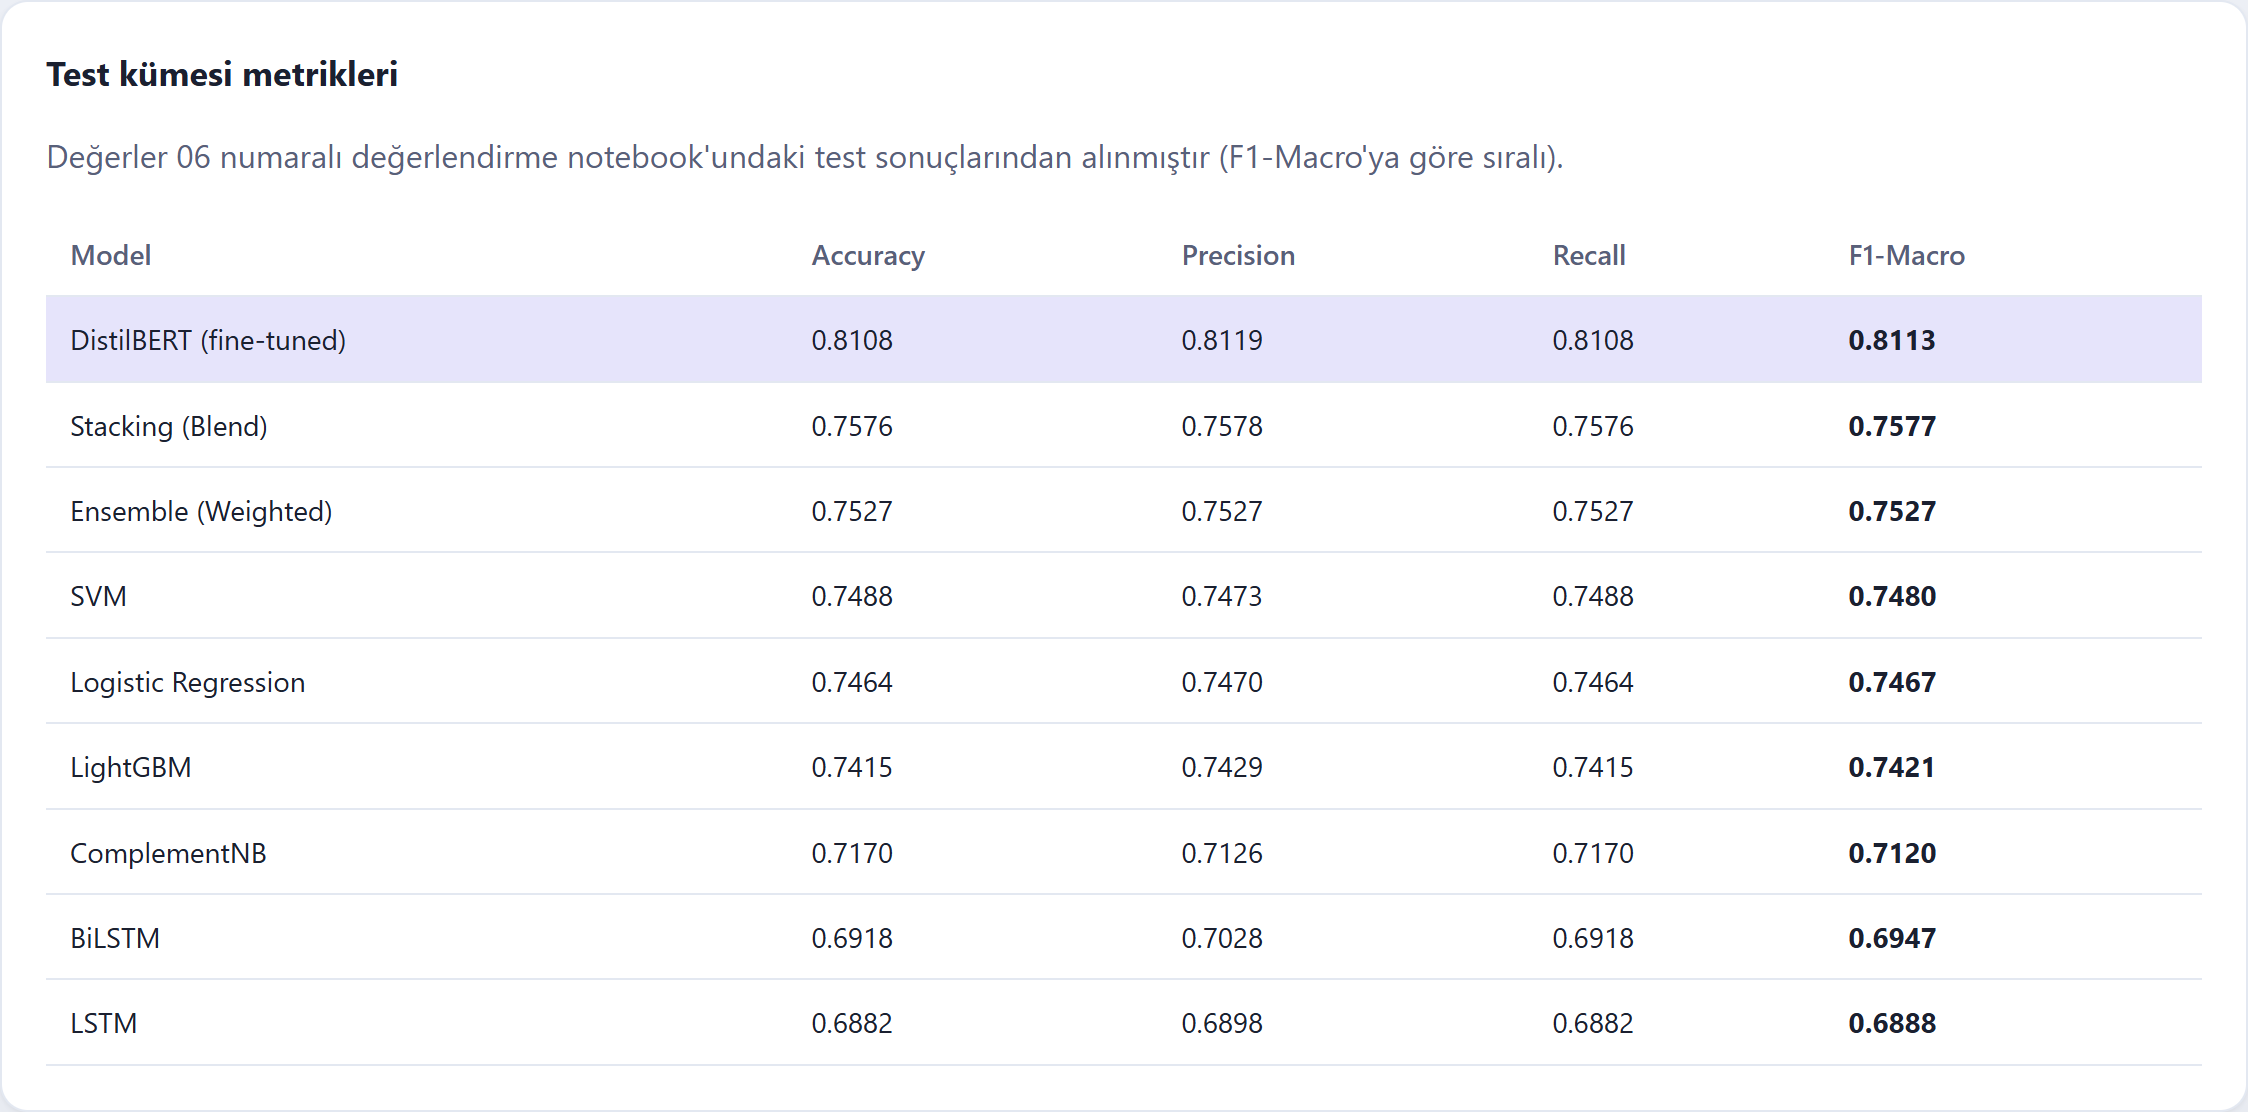
\includegraphics[width=\columnwidth,height=3.6cm,keepaspectratio]{11_leaderboard.png}
\caption{Web arayüzündeki test kümesi başarım tablosu; ince ayarlı DistilBERT en
üstte (0,8113).}
\label{fig:leaderboard}
\end{figure}

\begin{figure}[htbp]
\centering
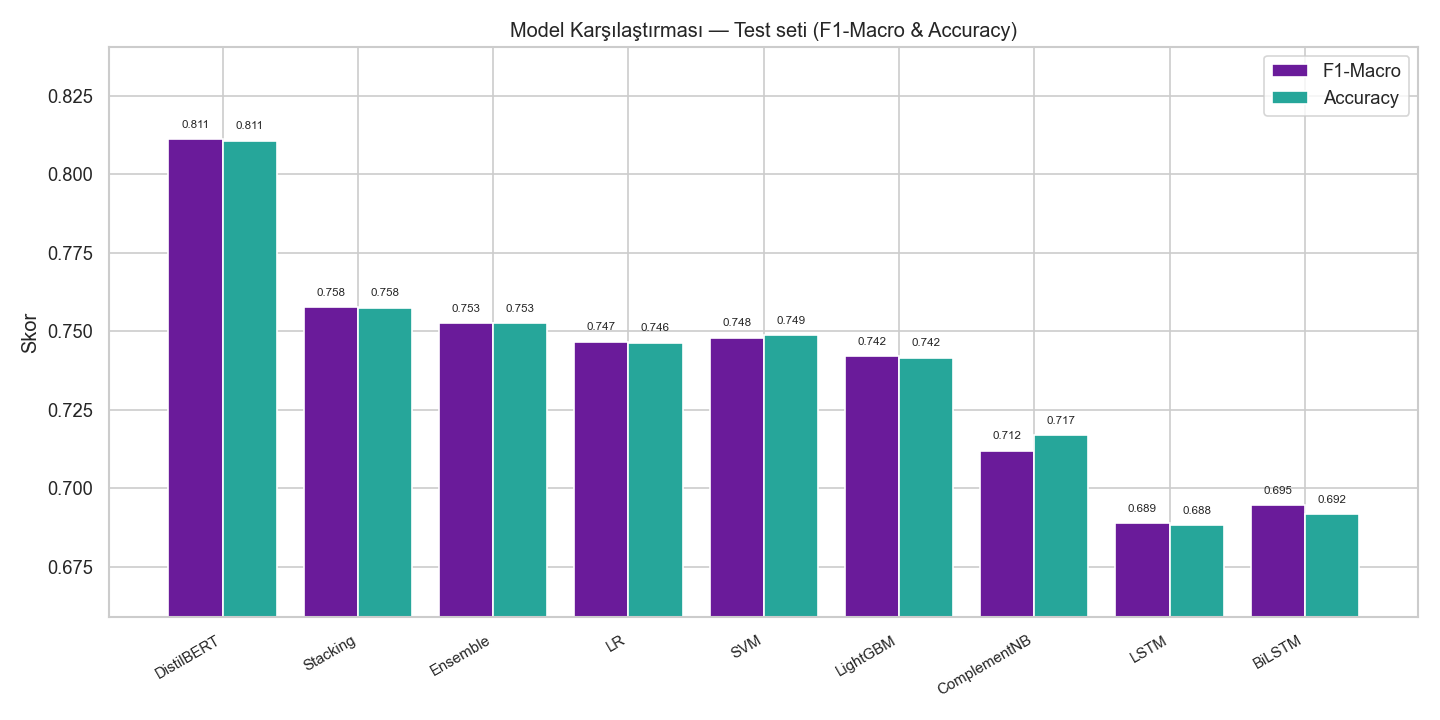
\includegraphics[width=\columnwidth,height=5cm,keepaspectratio]{14_model_comparison_final.png}
\caption{Test kümesinde modellerin F1-makro ve doğruluk karşılaştırması: ince ayarlı
DistilBERT (0,811) en yüksek; istifleme topluluğu (0,758) klasikler içinde önde;
sıfırdan eğitilen LSTM/BiLSTM geride kalır.}
\label{fig:f1}
\end{figure}

\begin{figure}[htbp]
\centering
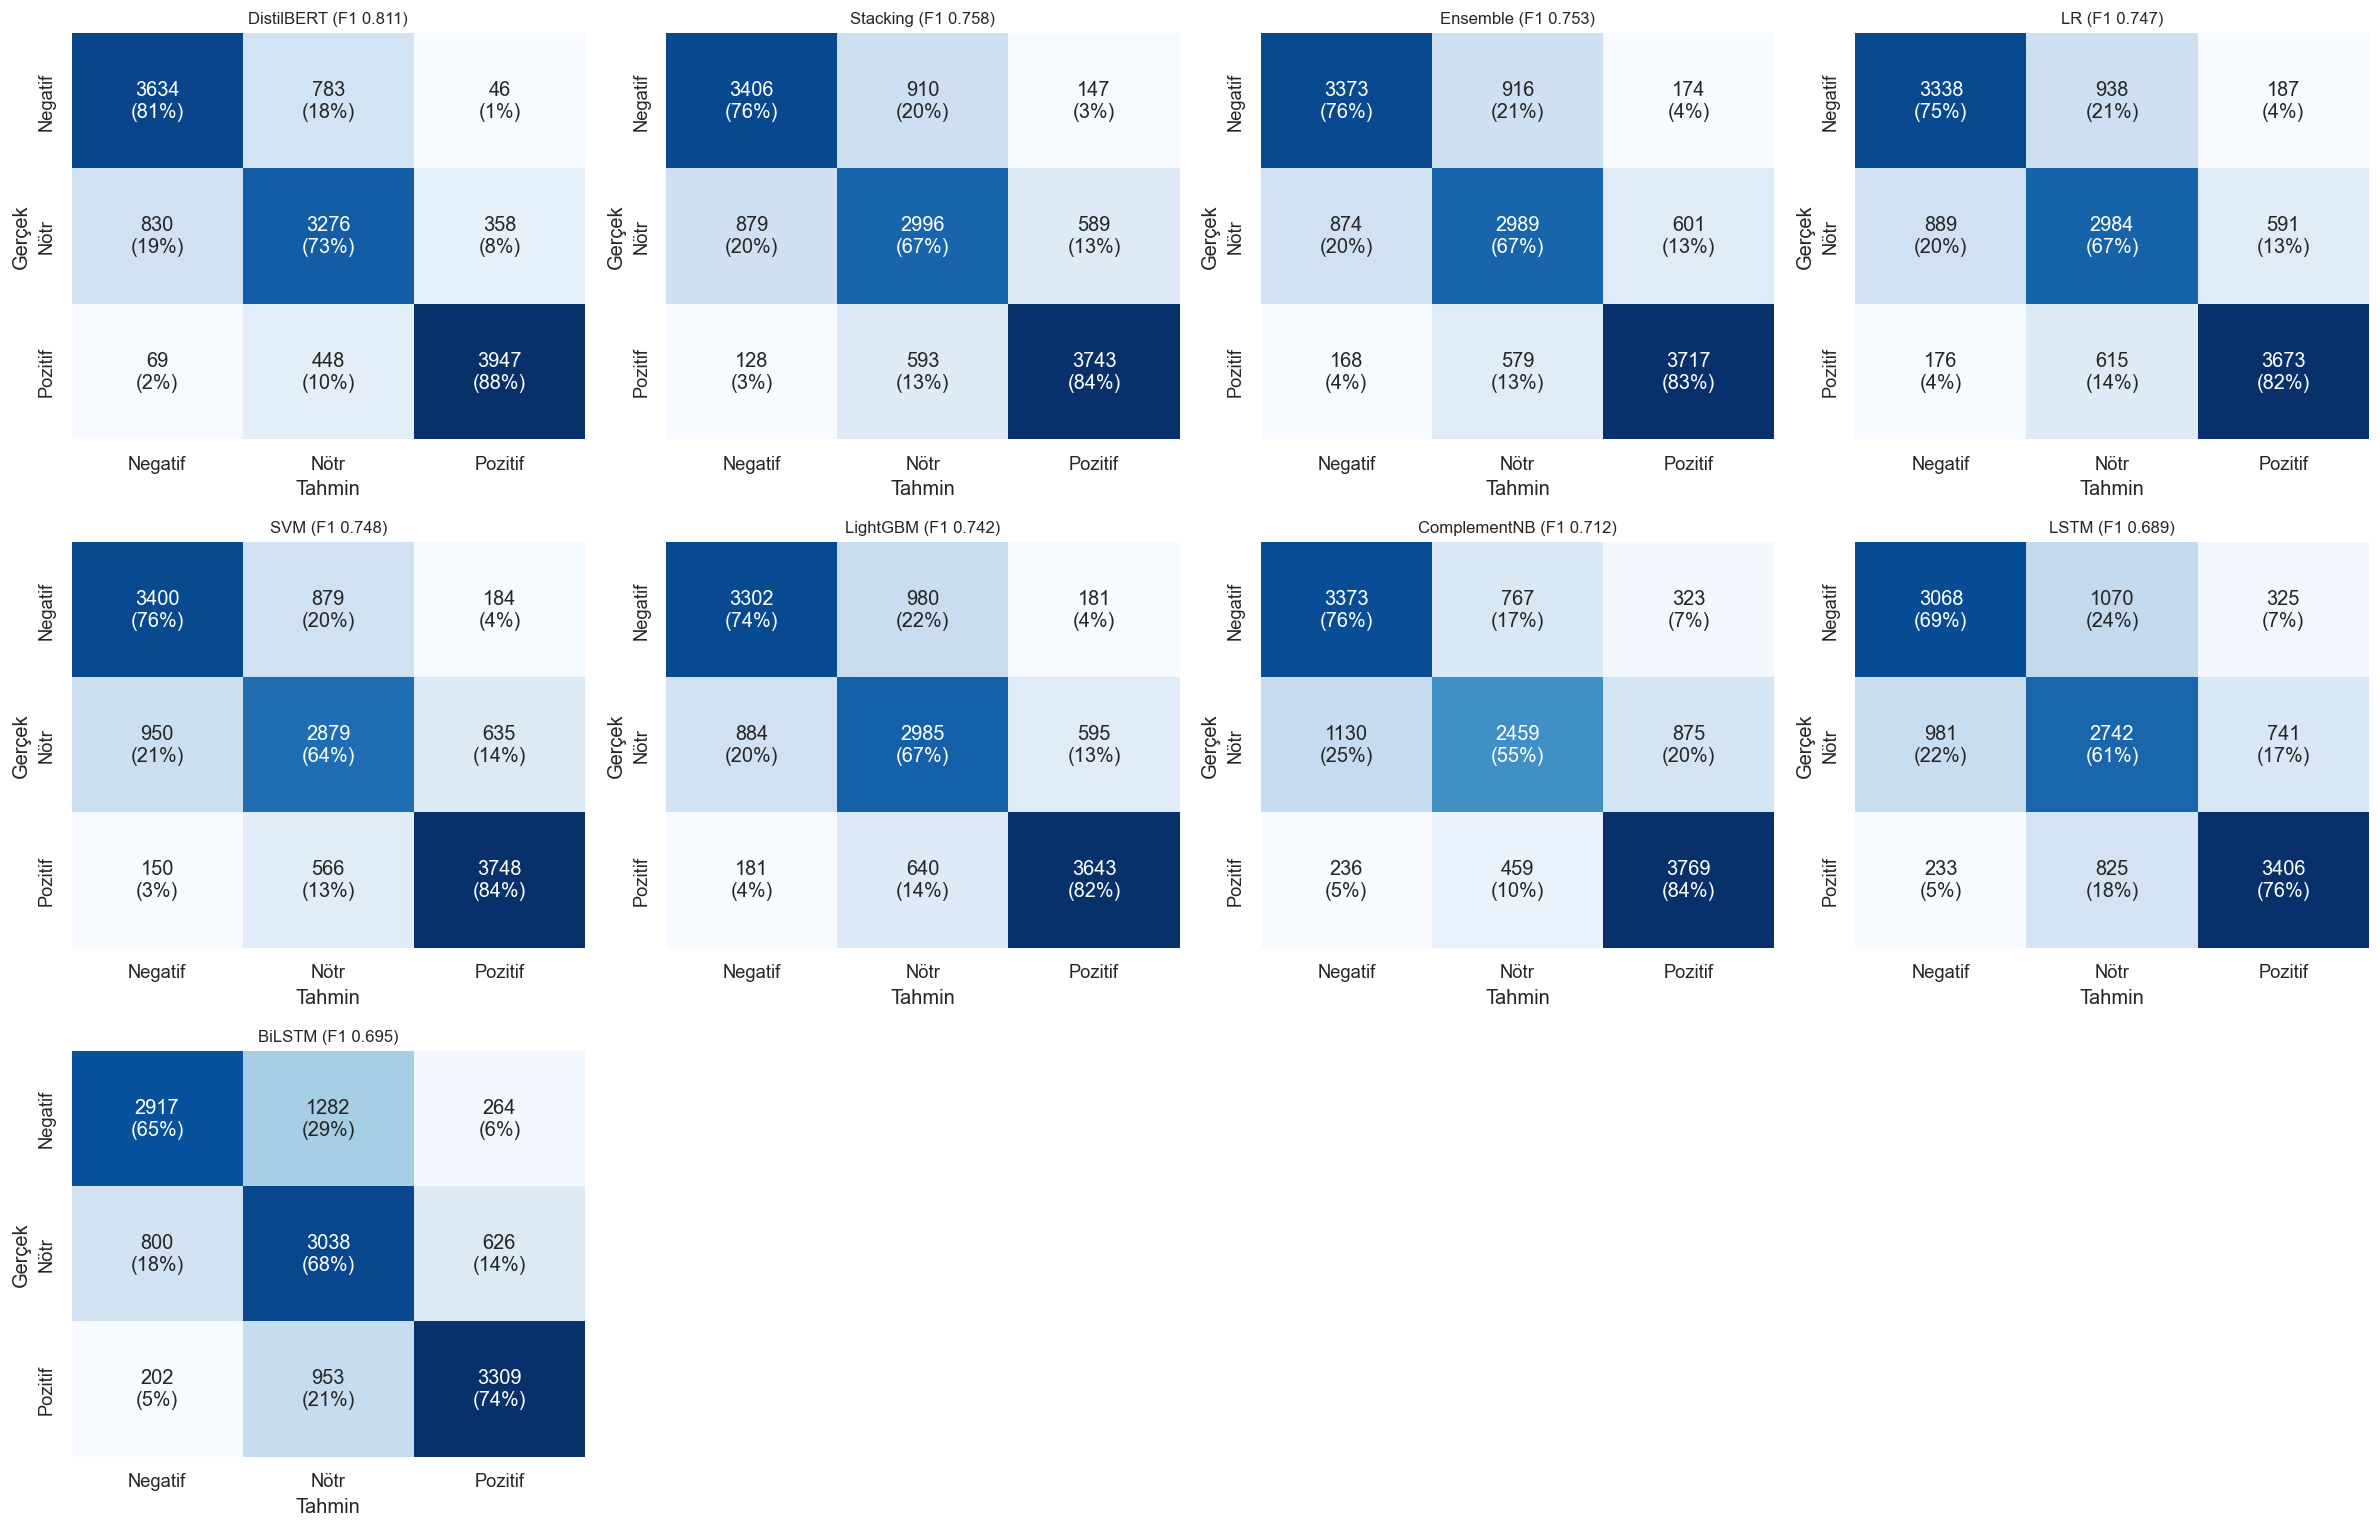
\includegraphics[width=\columnwidth,height=6.2cm,keepaspectratio]{15_confusion_all.png}
\caption{Tüm modeller için normalize karışıklık matrisleri (test). Nötr sınıfı tüm
modellerde en çok karıştırılan sınıftır; DistilBERT nötr ayrımında belirgin biçimde
daha başarılıdır.}
\label{fig:confusion}
\end{figure}

\subsection{İstatistiksel Anlamlılık ve Nötr Sınıf Analizi}
DistilBERT ile en iyi klasik model (istifleme) arasındaki farkın rastlantısal olup
olmadığını sınamak için eşli (paired) \textbf{McNemar testi} uygulanmıştır. Test
kümesinde yalnızca DistilBERT'in doğru bildiği 1.506 örneğe karşılık yalnızca
istiflemenin doğru bildiği 794 örnek vardır; süreklilik düzeltmeli
$\chi^2 = 219{,}8$, $p \approx 10^{-49}$. Bu, DistilBERT'in üstünlüğünün
istatistiksel olarak son derece anlamlı (rastlantı olmadığı) olduğunu gösterir.
Ayrıca, en çok karıştırılan \emph{nötr} sınıfı için DistilBERT olasılıklarına
\emph{yalnızca doğrulama kümesinde} sınıf-başına çarpan (eşik) ayarı uygulanmıştır;
bu, nötr duyarlılığını (recall) test kümesinde 0,734'ten \textbf{0,761}'e çıkarmış,
makro-F1'i ise pratikte değiştirmemiştir (model olasılıkları zaten iyi
dengelenmiştir). Eşik ayarı, nötr sınıfın zorluğunu nicelemek amacıyla
raporlanmış; varsayılan modelde kullanılmamıştır.

\subsection{Başlık (Summary) Ablation'ı}
Tablo~\ref{tab:ablation} ve Şekil~\ref{fig:ablation}, başlık bütünleştirmenin
etkisini gösterir. Başlık eklemek F1-makro skorunu model başına \dpos{+0,024} ile
\dpos{+0,029} arasında artırmıştır; topluluk için kazanç \dpos{+0,025}'tir. Düşük
maliyetli (yalnızca öznitelik metnini değiştiren) ama tüm modellerde tutarlı bu
iyileşme, başlık alanının taşıdığı duygu sinyalinin değerini doğrular.

\begin{table}[htbp]
\caption{Başlık (Summary) Ablation'ı (F1-Makro)}
\label{tab:ablation}
\centering
\small
\begin{tabular}{lccc}
\toprule
\textbf{Model} & \textbf{Yalnız Metin} & \textbf{Metin+Başlık} & \textbf{$\Delta$}\\
\midrule
Logistic Regression & 0,7203 & 0,7443 & \dpos{+0,0240}\\
SVM                 & 0,7171 & 0,7407 & \dpos{+0,0235}\\
LightGBM            & 0,7157 & 0,7451 & \dpos{+0,0293}\\
\textbf{Ensemble}   & 0,7258 & \textbf{0,7512} & \dpos{+0,0254}\\
\bottomrule
\end{tabular}
\end{table}

\begin{figure}[htbp]
\centering
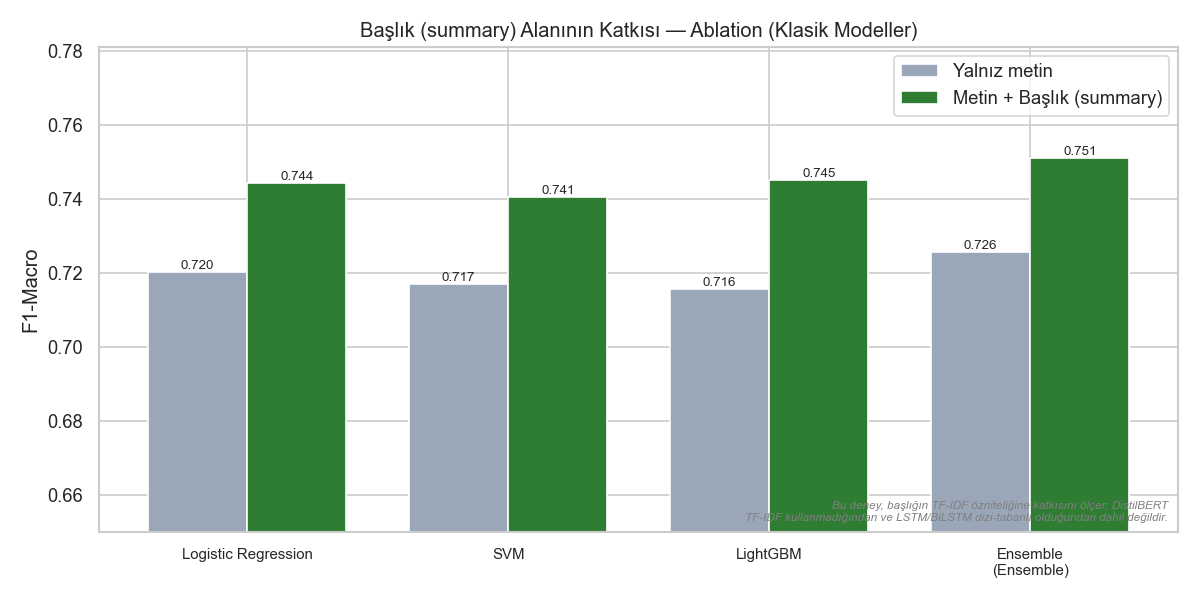
\includegraphics[width=0.72\columnwidth,height=4.4cm,keepaspectratio]{08_ablation.png}
\caption{Başlık alanının katkısı: her modelde gövde+başlık (yeşil), yalnız
gövdeyi (gri) geçer.}
\label{fig:ablation}
\end{figure}

\subsection{Topluluk Analizi}
İstifleme (stacking) topluluğu, en iyi \emph{tekil} klasik modeli (SVM, 0,7480)
geçerek klasik modeller arasında en yüksek skoru (\textbf{0,7577}) elde etmiştir;
ağırlıklı oylamadan (0,7527) da üstündür. Meta-modelin doğrulama olasılıklarıyla
eğitilmesi (taban modellerin eğitim olasılıklarıyla değil) bu kazancın
\emph{sızıntısız} ve gerçek olmasını güvence altına alır. Genel sıralamada ise
DistilBERT (0,8113) bu klasik tavanı da açık farkla aşmıştır.
Şekil~\ref{fig:sonuc}, ``Awful, do not buy'' başlıklı olumsuz bir yorumun yüksek
güvenle Negatif sınıflandırıldığı örnek bir çıkarımı; Şekil~\ref{fig:tum} ise tüm
modellerin aynı metin için aynı kararı verdiğini gösterir.

\begin{figure}[htbp]
\centering
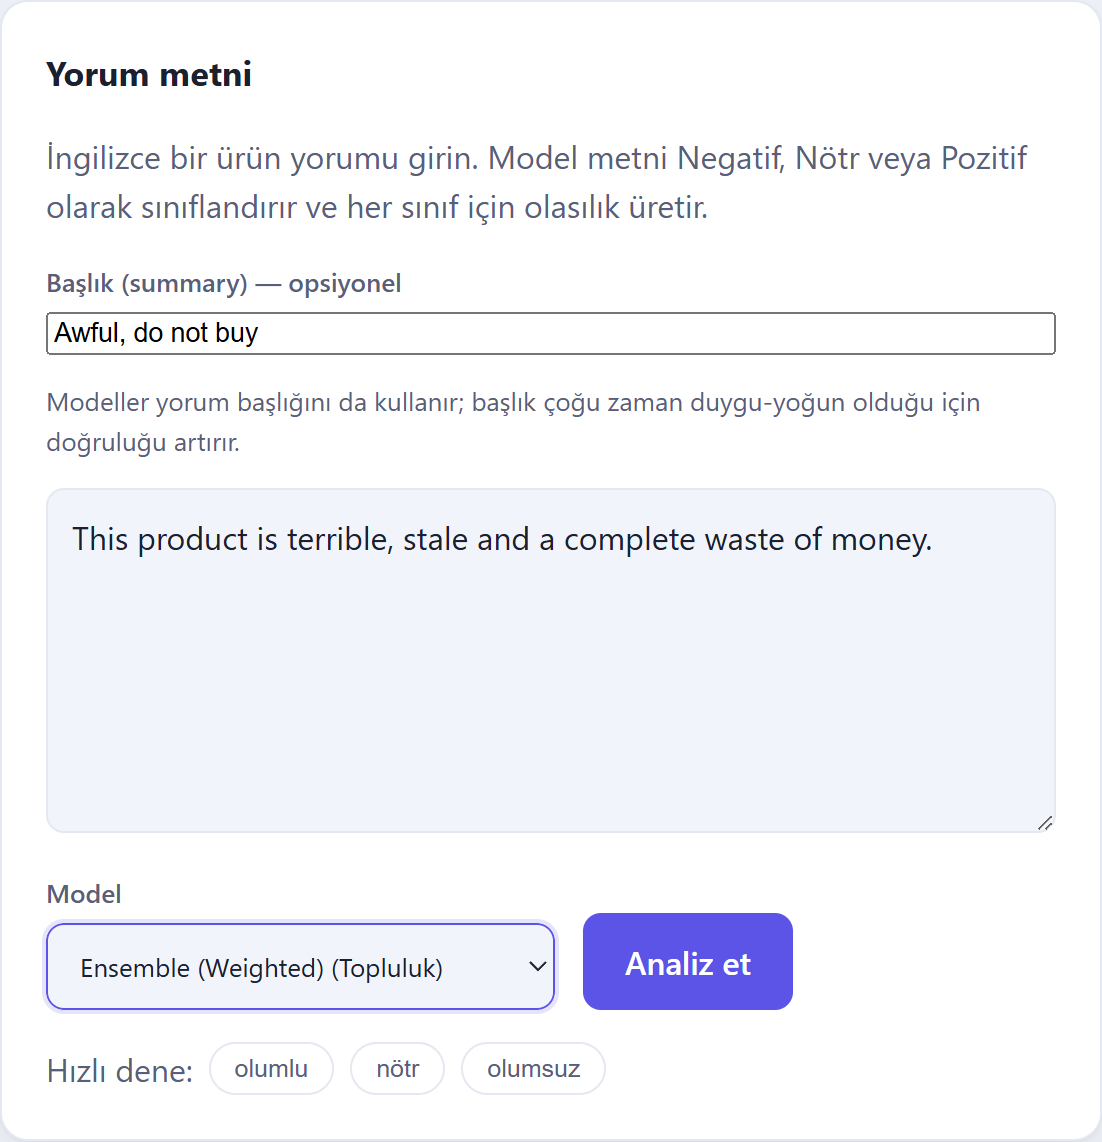
\includegraphics[width=0.55\columnwidth,height=5cm,keepaspectratio]{09_giris_kart.png}
\caption{Tekli tahmin giriş kartı: opsiyonel başlık (summary) alanı ve model seçimi.}
\label{fig:giris}
\end{figure}

\begin{figure}[htbp]
\centering
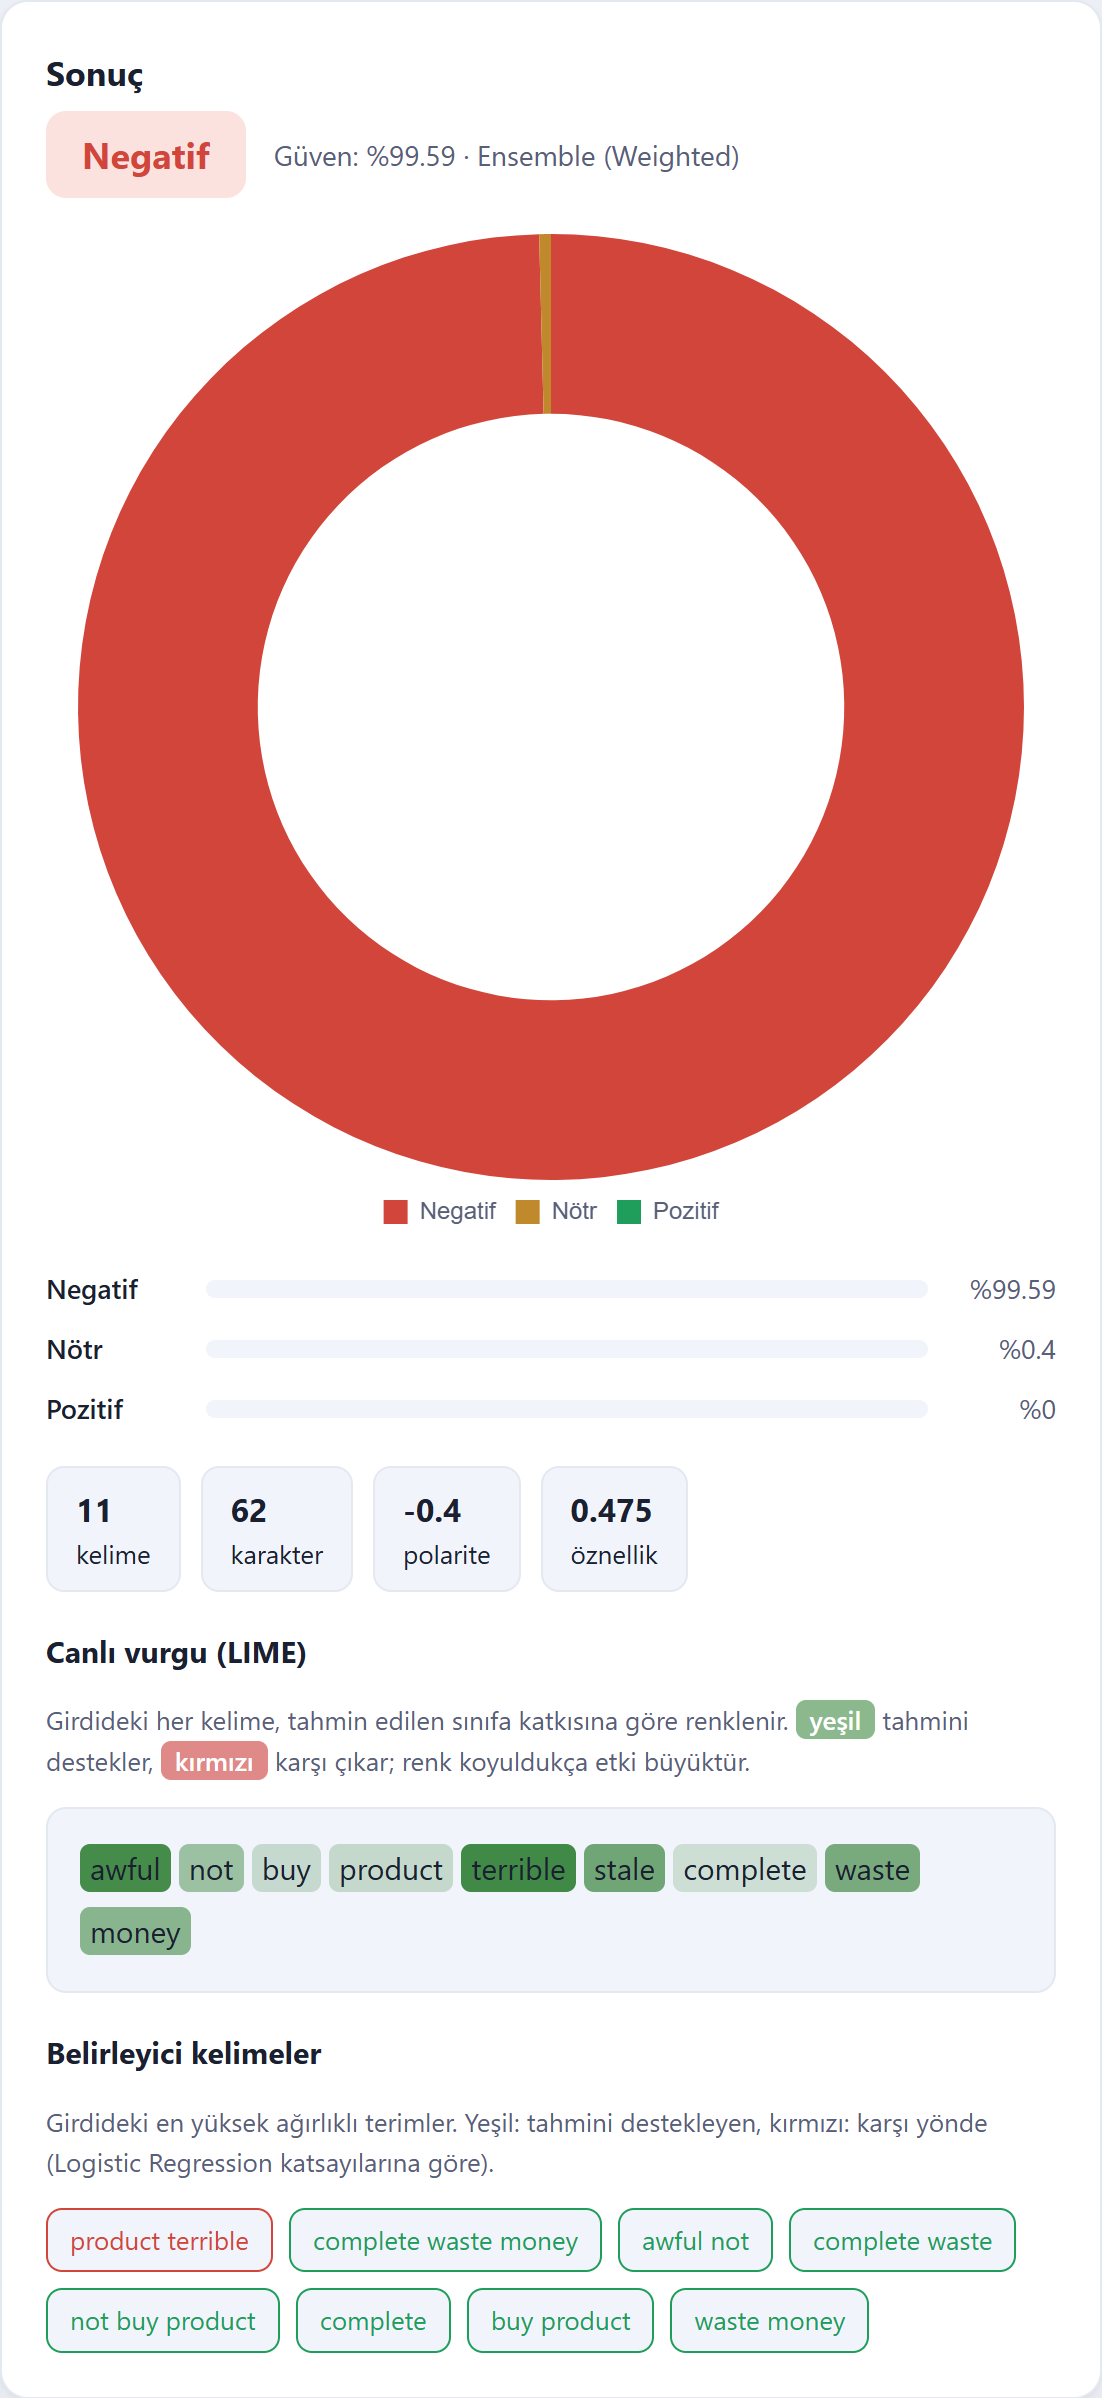
\includegraphics[width=0.5\columnwidth,height=5.5cm,keepaspectratio]{06_sonuc_karti.png}
\caption{Sonuç kartı: sınıf olasılıkları, metin istatistikleri ve kelime düzeyinde
canlı açıklama.}
\label{fig:sonuc}
\end{figure}

\begin{figure}[htbp]
\centering
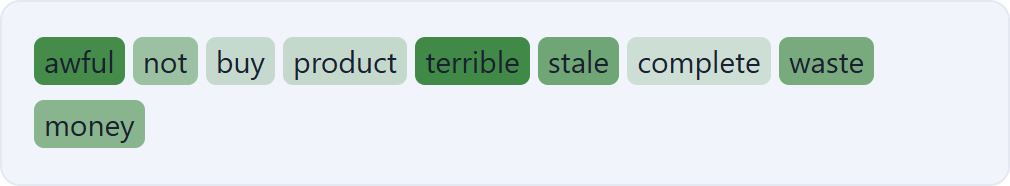
\includegraphics[width=0.9\columnwidth,height=2cm,keepaspectratio]{07_lime_yakin.png}
\caption{Canlı LIME vurgusu: ``terrible'' ve ``awful'' en güçlü Negatif katkıyı sağlar.}
\label{fig:lime}
\end{figure}

\begin{figure}[htbp]
\centering
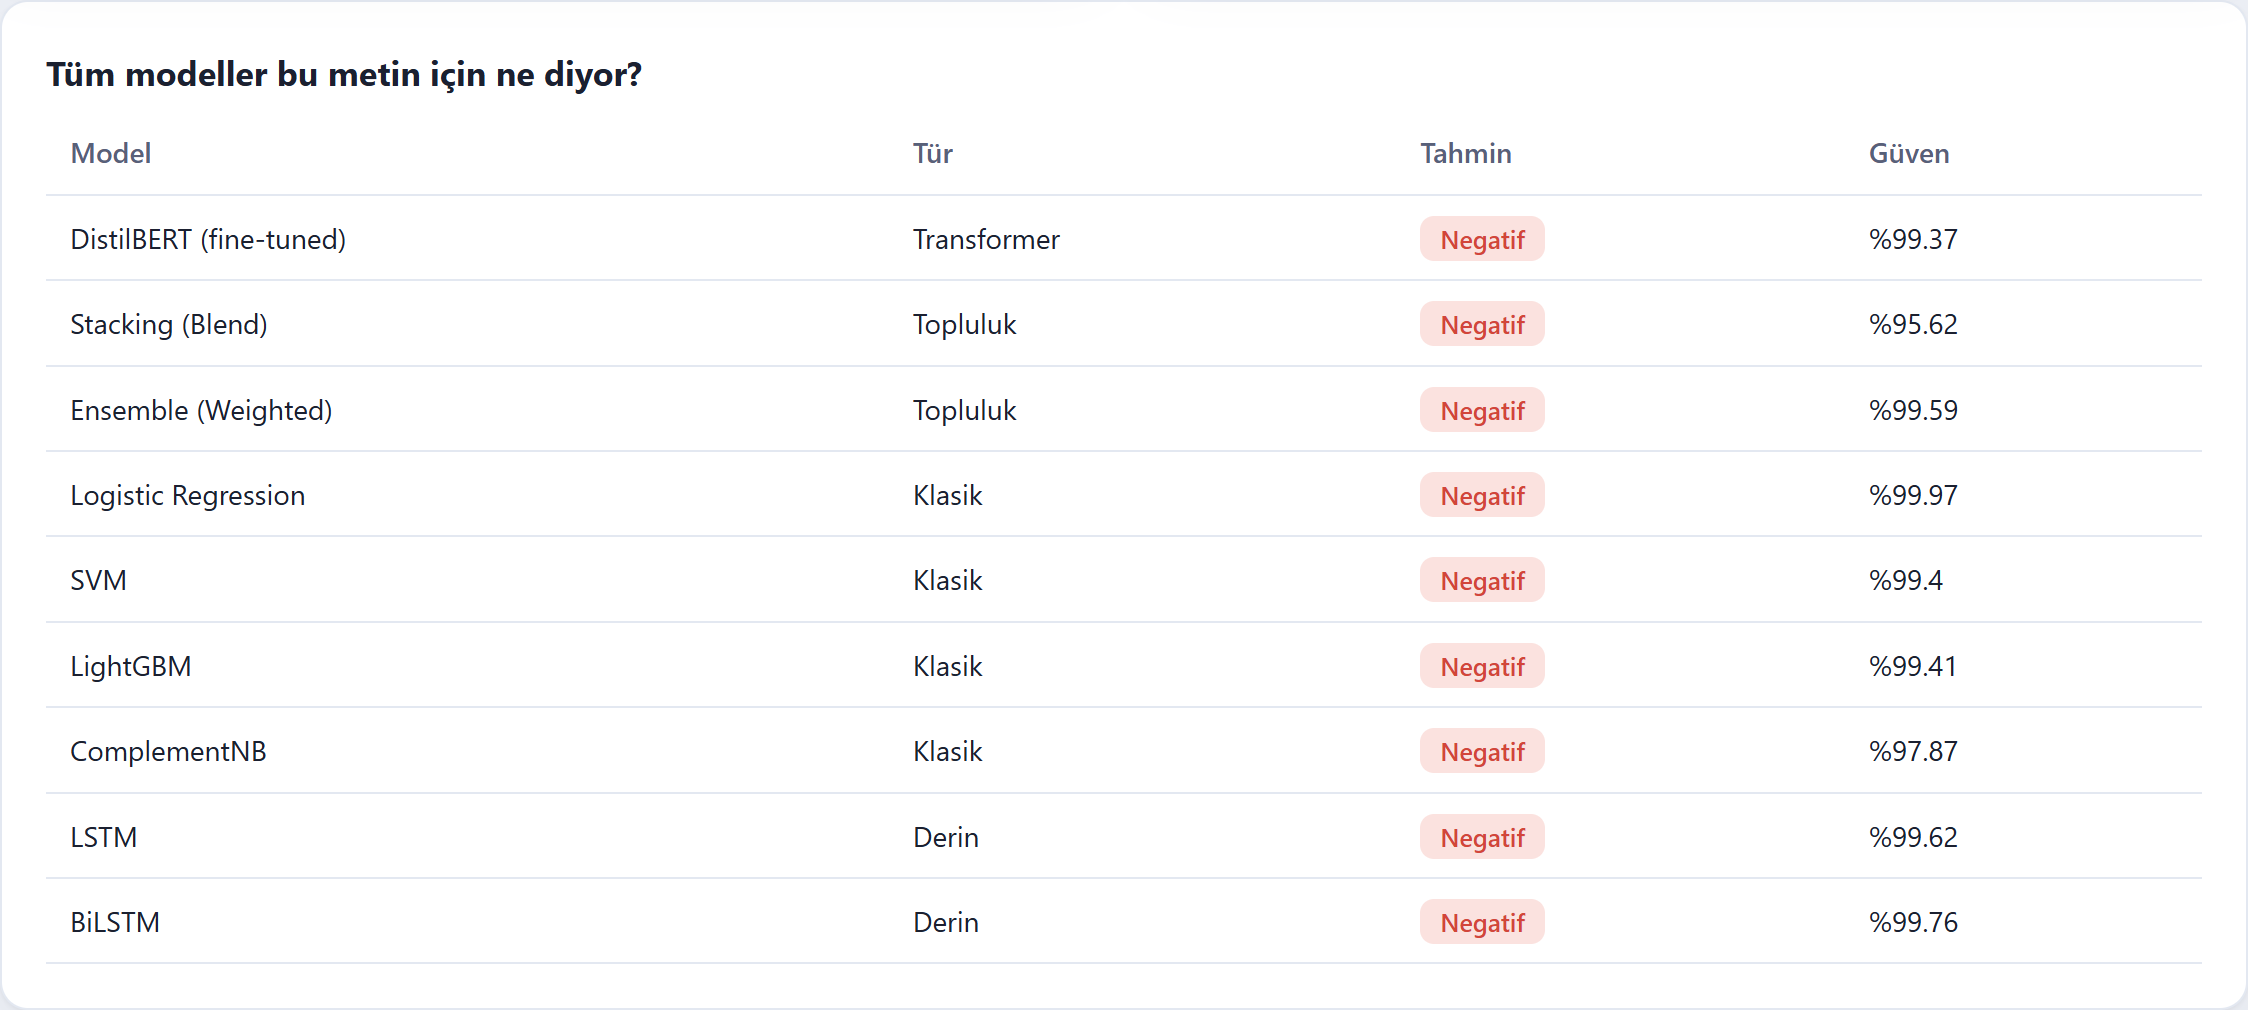
\includegraphics[width=\columnwidth,height=3.2cm,keepaspectratio]{10_tum_modeller.png}
\caption{Aynı girdi için tüm modellerin kararı; DistilBERT ve topluluklar dâhil
dokuz model.}
\label{fig:tum}
\end{figure}

\subsection{Sözlük-Dışı (OOV) Kelimeler}
Geliştirme sırasında gözlemlenen ilginç bir durum, bazı bariz olumsuz kelimelerin
(ör. ``shit'') tek başına girildiğinde TF-IDF tarafında karşılık bulamamasıdır.
İnceleme, bu kelimenin veri kümesinde yalnızca 9 dokümanda geçtiğini ve
\texttt{max\_features=50000} frekans tavanının altında kaldığı için sözlüğe
alınmadığını göstermiştir. Bu bir kusur değil, bir gıda yorumu kümesinin doğal
sonucudur: kullanıcılar küfür yerine ``awful'', ``terrible'', ``disgusting''
ifadelerini tercih eder. Buna rağmen sistemin doğru (Negatif) tahmin üretmesi
(Şekil~\ref{fig:oov}), TF-IDF dışındaki \textbf{sayısal duygu özniteliklerinin}
(TextBlob polaritesi) modele dayanıklılık kazandırdığını gösterir. Canlı açıklama
bu kelimeyi ``bilinmiyor'' olarak işaretleyerek şeffaflık sağlar.

\begin{figure}[htbp]
\centering
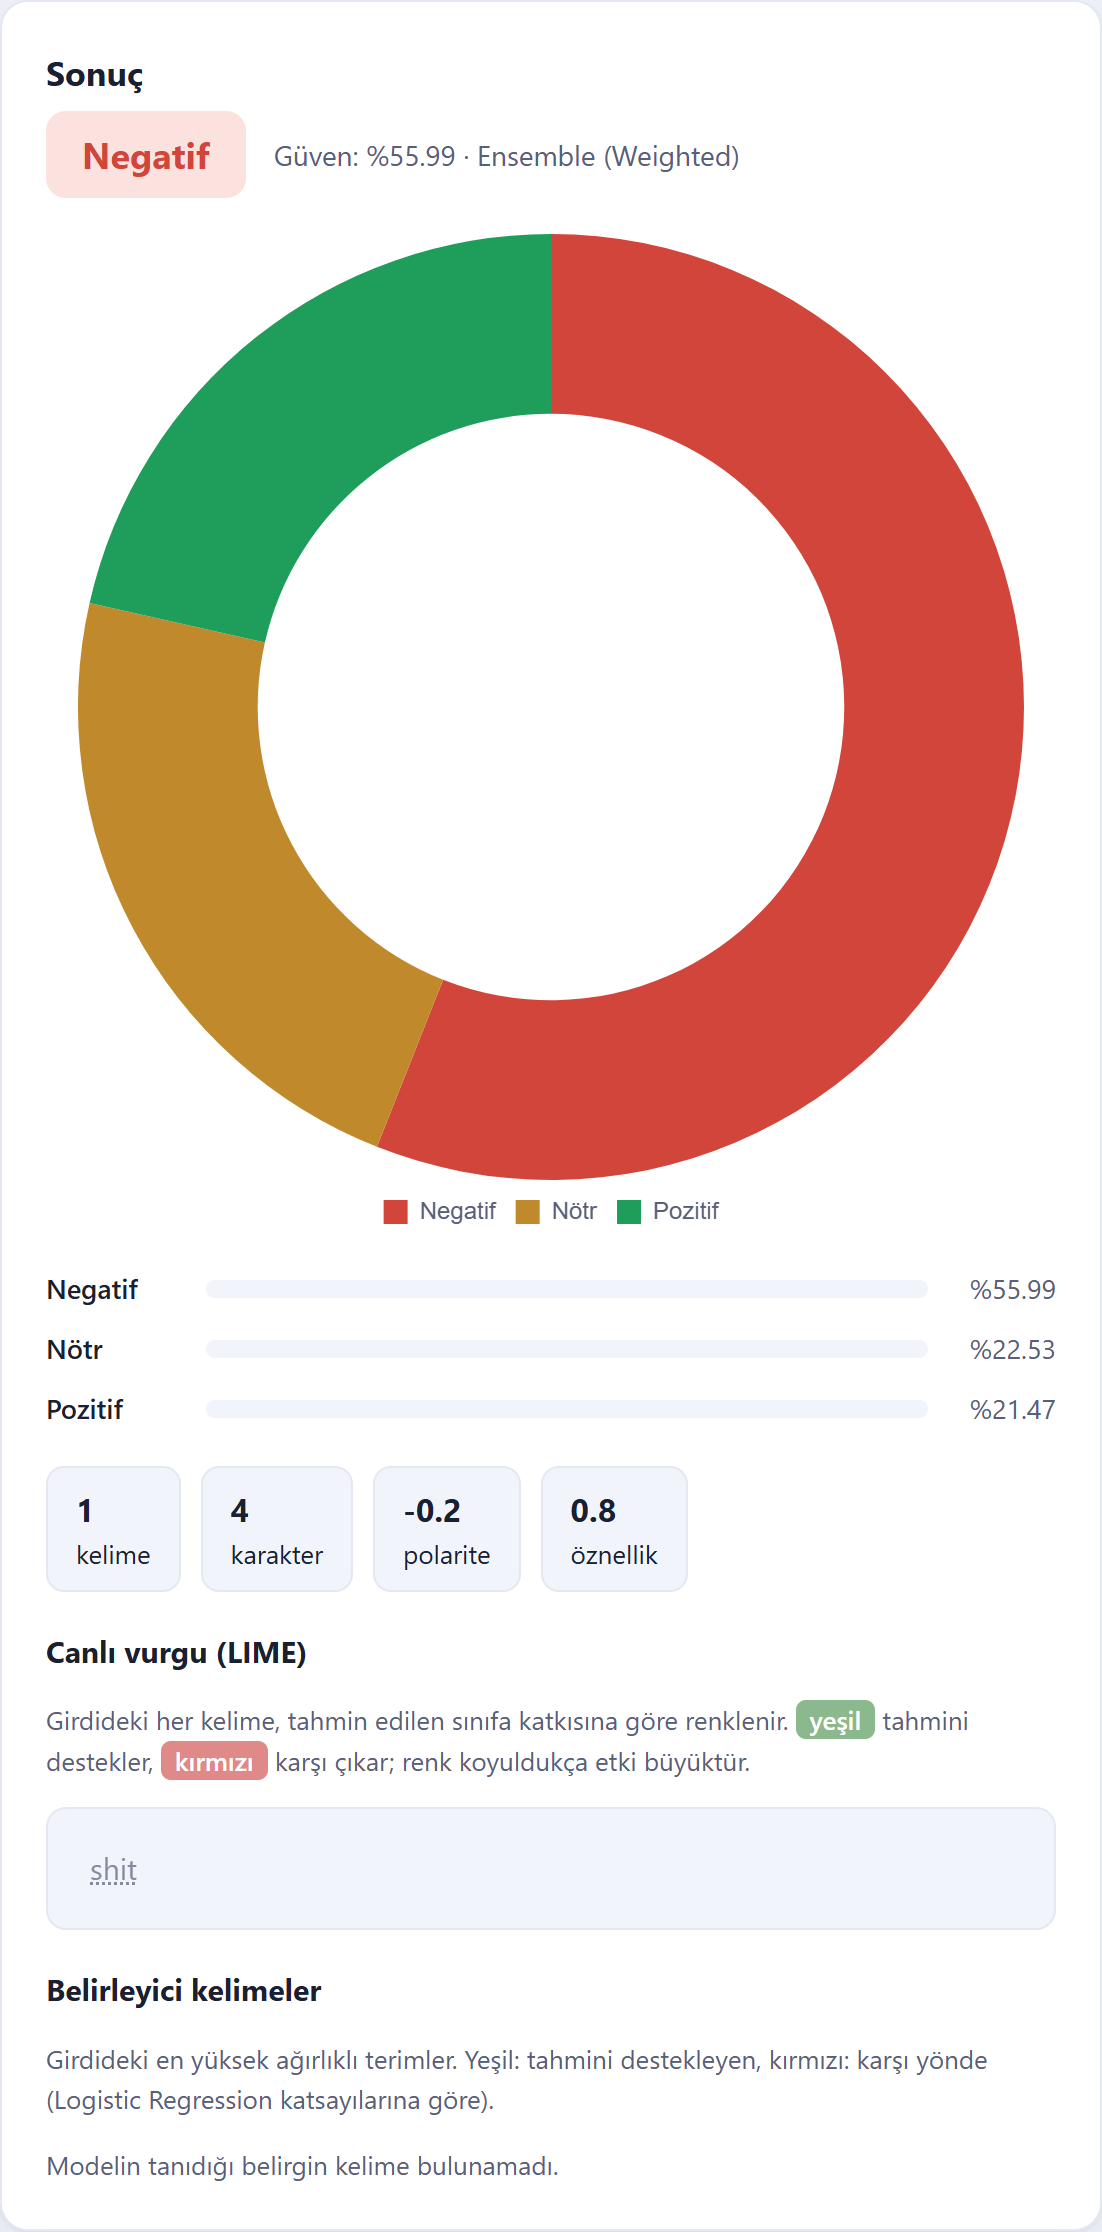
\includegraphics[width=0.5\columnwidth,height=4cm,keepaspectratio]{13_oov_kart.png}
\caption{Sözlük-dışı (OOV) örnek: yalnızca ``shit'' girildiğinde kelime sözlükte
olmamasına rağmen sayısal duygu öznitelikleri sayesinde Negatif tahmin edilir.}
\label{fig:oov}
\end{figure}

\subsection{Klasik vs. Derin Modeller}
Derin modellerin geride kalması iki nedene bağlanabilir: (i) hesaplama bütçesi
nedeniyle yalnızca 45.000 örnekle eğitilmeleri; (ii) kısa metinlerde n-gram
TF-IDF'in zaten güçlü ayırt edicilik sunması. Sıfırdan öğrenilen 64 boyutlu
gömüler, sınırlı veriyle zengin anlamsal temsiller oluşturmakta yetersiz
kalmaktadır.

%================================================================== IX. Arayuz
\section{Web Arayüzü}
Tüm bileşenler Flask tabanlı etkileşimli bir web arayüzünde toplanmıştır.
Arayüz; \emph{tekli tahmin} (opsiyonel başlık alanı, model seçimi, olasılık
grafiği ve canlı LIME açıklaması---Şekil~\ref{fig:giris}), \emph{toplu analiz},
\emph{model karşılaştırma} (Şekil~\ref{fig:leaderboard}--\ref{fig:f1}) ve
\emph{keşifsel analiz} sayfalarını sunar. Tekli tahmin ekranında, seçilen modelin
kararının yanı sıra \emph{tüm} modellerin aynı metin için verdiği kararlar da
gösterilerek karşılaştırmalı bir bakış sağlanır (Şekil~\ref{fig:tum}). Giriş ekranı
Şekil~\ref{fig:giris}, sonuç kartı Şekil~\ref{fig:sonuc}, başarım tablosu ise
Şekil~\ref{fig:leaderboard}'de gösterilmiştir.

%================================================================== X. Sinirliliklar
\section{Sınırlılıklar ve Gelecek Çalışmalar}
Sistem yalnızca İngilizce yorumlar için tasarlanmıştır; nötr sınıf, doğası gereği
en çok karıştırılan sınıftır ve genel başarımı sınırlayan başlıca etmendir. Canlı
açıklama, basitlik için Lojistik Regresyon katsayılarına dayanır; seçilen model
DistilBERT olsa dahi kelime önemi LR üzerinden gösterilir---bu, BERT için doğrudan
bir açıklama olmadığından bir sınırlılıktır. DistilBERT yalnızca CPU ve dengeli
62.486 örnekle, iki dönem eğitilmiştir; daha fazla veri/dönem ve GPU ile başarımın
bir miktar daha artması olasıdır. Gelecek çalışmalarda: (i) daha güçlü veya duyguya
özel önceden eğitilmiş Transformer'lar (RoBERTa, BERT-base) ile başarımın daha da
yükseltilmesi; (ii) DistilBERT'in de katıldığı klasik+Transformer toplulukları;
(iii) DistilBERT'e özgü dikkat (attention)/SHAP tabanlı açıklamalar; (iv) çok dilli
(Türkçe dâhil) desteğin eklenmesi hedeflenmektedir.

%================================================================== XI. Sonuc
\section{Sonuç}
Bu çalışma, Amazon ürün yorumları için üç sınıflı, uçtan uca ve açıklanabilir bir
duygu analizi sistemi sunmuştur. Önerilen geliştirmeler---başlık bütünleştirme,
istifleme (stacking) topluluğu, canlı LIME açıklaması ve önceden eğitilmiş bir
Transformer'ın (DistilBERT) ince ayarlanması---birlikte hem doğruluğu hem de
yorumlanabilirliği belirgin biçimde artırmıştır. Sızıntısı giderilmiş istifleme
topluluğu klasik modeller arasında \textbf{0,7577 F1-makro} ile en iyi olurken,
ince ayarlı DistilBERT \textbf{0,8113 F1-makro} ile tüm modelleri geçerek genel en
iyi sonucu vermiş; önceki temel modele göre \textbf{$+6$ F1 puanı} kazanç
sağlanmıştır. Ayrıca öznitelik çıkarımındaki bir veri sızıntısı giderilip tüm model
seçimleri yalnızca doğrulama kümesinde yapılarak değerlendirmenin güvenilirliği
güçlendirilmiştir. Sonuçlar iki tamamlayıcı bulguyu ortaya koyar: iyi tasarlanmış
klasik öznitelik mühendisliği ve hafif topluluk yöntemleri, sınırlı veri/hesaplama
koşullarında sıfırdan eğitilen derin dizi modellerine kıyasla güçlü, hızlı ve
yorumlanabilir bir taban sunar; buna karşılık, aktarım öğrenmesiyle gelen önceden
eğitilmiş bir Transformer'ın ince ayarı, bu tabanı aşan en yüksek başarımı sağlar.

%------------------------------------------------------------------ Kaynaklar
\begin{thebibliography}{9}
\bibitem{mcauley} J. McAuley and J. Leskovec, ``From amateurs to connoisseurs:
modeling the evolution of user expertise through online reviews,'' in
\emph{Proc. Int. Conf. World Wide Web (WWW)}, 2013, pp. 897--908.
\bibitem{pang} B. Pang and L. Lee, ``Opinion mining and sentiment analysis,''
\emph{Found. Trends Inf. Retr.}, vol. 2, no. 1--2, pp. 1--135, 2008.
\bibitem{sklearn} F. Pedregosa \emph{et al.}, ``Scikit-learn: Machine learning in
Python,'' \emph{J. Mach. Learn. Res.}, vol. 12, pp. 2825--2830, 2011.
\bibitem{lgbm} G. Ke \emph{et al.}, ``LightGBM: A highly efficient gradient
boosting decision tree,'' in \emph{Adv. Neural Inf. Process. Syst. (NeurIPS)},
2017, pp. 3146--3154.
\bibitem{lstm} S. Hochreiter and J. Schmidhuber, ``Long short-term memory,''
\emph{Neural Comput.}, vol. 9, no. 8, pp. 1735--1780, 1997.
\bibitem{lime} M. T. Ribeiro, S. Singh, and C. Guestrin, ```Why should I trust
you?': Explaining the predictions of any classifier,'' in \emph{Proc. ACM SIGKDD},
2016, pp. 1135--1144.
\bibitem{svm} T. Joachims, ``Text categorization with support vector machines:
Learning with many relevant features,'' in \emph{Proc. ECML}, 1998, pp. 137--142.
\bibitem{distilbert} V. Sanh, L. Debut, J. Chaumond, and T. Wolf, ``DistilBERT, a
distilled version of BERT: smaller, faster, cheaper and lighter,'' in
\emph{NeurIPS EMC\textsuperscript{2} Workshop}, 2019.
\bibitem{bert} J. Devlin, M.-W. Chang, K. Lee, and K. Toutanova, ``BERT:
Pre-training of deep bidirectional transformers for language understanding,'' in
\emph{Proc. NAACL-HLT}, 2019, pp. 4171--4186.
\end{thebibliography}

\end{document}
